\documentclass[12pt,]{article}
\usepackage{lmodern}
\usepackage{amssymb,amsmath}
\usepackage{ifxetex,ifluatex}
\usepackage{fixltx2e} % provides \textsubscript
\ifnum 0\ifxetex 1\fi\ifluatex 1\fi=0 % if pdftex
  \usepackage[T1]{fontenc}
  \usepackage[utf8]{inputenc}
\else % if luatex or xelatex
  \ifxetex
    \usepackage{mathspec}
  \else
    \usepackage{fontspec}
  \fi
  \defaultfontfeatures{Ligatures=TeX,Scale=MatchLowercase}
  \newcommand{\euro}{€}
    \setmainfont[]{Times New Roman}
\fi
% use upquote if available, for straight quotes in verbatim environments
\IfFileExists{upquote.sty}{\usepackage{upquote}}{}
% use microtype if available
\IfFileExists{microtype.sty}{%
\usepackage{microtype}
\UseMicrotypeSet[protrusion]{basicmath} % disable protrusion for tt fonts
}{}
\usepackage[margin=1in]{geometry}
\usepackage{hyperref}
\PassOptionsToPackage{usenames,dvipsnames}{color} % color is loaded by hyperref
\hypersetup{unicode=true,
            pdftitle={Convolutional Neural Network based Classification of Histopathologic Neoplastic Tissue Images},
            pdfauthor={Aadi Kalloo},
            pdfborder={0 0 0},
            breaklinks=true}
\urlstyle{same}  % don't use monospace font for urls
\usepackage{longtable,booktabs}
\usepackage{graphicx,grffile}
\makeatletter
\def\maxwidth{\ifdim\Gin@nat@width>\linewidth\linewidth\else\Gin@nat@width\fi}
\def\maxheight{\ifdim\Gin@nat@height>\textheight\textheight\else\Gin@nat@height\fi}
\makeatother
% Scale images if necessary, so that they will not overflow the page
% margins by default, and it is still possible to overwrite the defaults
% using explicit options in \includegraphics[width, height, ...]{}
\setkeys{Gin}{width=\maxwidth,height=\maxheight,keepaspectratio}
\setlength{\parindent}{0pt}
\setlength{\parskip}{6pt plus 2pt minus 1pt}
\setlength{\emergencystretch}{3em}  % prevent overfull lines
\providecommand{\tightlist}{%
  \setlength{\itemsep}{0pt}\setlength{\parskip}{0pt}}
\setcounter{secnumdepth}{5}

%%% Use protect on footnotes to avoid problems with footnotes in titles
\let\rmarkdownfootnote\footnote%
\def\footnote{\protect\rmarkdownfootnote}

%%% Change title format to be more compact
\usepackage{titling}

% Create subtitle command for use in maketitle
\newcommand{\subtitle}[1]{
  \posttitle{
    \begin{center}\large#1\end{center}
    }
}

\setlength{\droptitle}{-2em}
  \title{Convolutional Neural Network based Classification of Histopathologic
Neoplastic Tissue Images}
  \pretitle{\vspace{\droptitle}\centering\huge}
  \posttitle{\par}
  \author{Aadi Kalloo}
  \preauthor{\centering\large\emph}
  \postauthor{\par}
  \predate{\centering\large\emph}
  \postdate{\par}
  \date{December 11 2017}


% Redefines (sub)paragraphs to behave more like sections
\ifx\paragraph\undefined\else
\let\oldparagraph\paragraph
\renewcommand{\paragraph}[1]{\oldparagraph{#1}\mbox{}}
\fi
\ifx\subparagraph\undefined\else
\let\oldsubparagraph\subparagraph
\renewcommand{\subparagraph}[1]{\oldsubparagraph{#1}\mbox{}}
\fi

\usepackage{setspace}
\doublespacing
\setlength\parindent{24pt}
\usepackage{float}

\begin{document}
\maketitle

{
\setcounter{tocdepth}{3}
\tableofcontents
}
\newpage

\section{Introduction}\label{introduction}

The diagnosis of cancers in modern medicine typically involves a biopsy
of the tissue in question followed by visual microscopic examination by
a licensed pathologist, after biopsy specimens have been sectioned and
placed onto glass slides (McKenney, 2017). Pathologists often use both
permanent and diagnostic slides to aid in their analysis of the biopsied
tissue. The diagnostic slides are obtained by slicing fresh tissue from
the sample on a microtome. The pathologist will then confirm with the
surgeon about the cancer diagnosis, often when the patient is still in
surgery. The biopsied tissue undergoes a different procedure for the
making of permanent slides: the tissue is fixed in formalin, water is
removed by a machine and replaced with paraffin wax, and the tissue is
then cut into thin slices using a microtome and places on slides
(Culling, Allison, \& Barr, 2014). To visualize the tissue under a
microscope, the sections are stained with one or possibly multiple
pigments. The aim of staining is to reveal cellular components, while
counterstains are used to provide contrast (Gurcan et al., 2009).

Given that human pathologists can reach conclusions based on the
physical features of the tissue sample (i.e.~cell morphology, presence
of artifacts), it follows that computer models can be trained to detect
features in a similar manner. The visual nature of this method gives way
to improvements in efficiency through automation, particularly through
the use of computer vision algorithms. One recent example of this
ideology put into practice is the development of a Convolutional Neural
Network (CNN) that can produce dermatologist-level accuracy in the
classification of skin cancer images (Esteva et al., 2017). That project
built upon previous technological developments in neural network
architecture by utilizing a network structure developed by Google Inc.
named Inception v3 (Szegedy et al., 2016). By taking advantage of this
architecture with weights pre-trained from the ImageNet data set,
significant developments in multi-class recognition of dermatological
lesions was achieved. Another CNN is the ConvNet with 19 weight layers,
allowing for deep visual recognition on a large scale. VGG19 is the
improved model of the ConvNet-19 used in the ILSVRC-2014 competition,
and is used in numerous image recognition data sets (Simonyan \&
Zisserman, 2014).

While there has been much progress recently in computer-aided diagnosis
in areas of medicine including radiology and dermatology, there have
been fewer efforts in the development of algorithms that can effectively
classify histopathology slides. Technologically focused works in the
area of histology have focused primarily on a single cancer type
(Cireşan et al., 2013; Xu et al., 2016); it is likely that work in this
arena has been limited by the availability of high quality data sets. To
date, no published works have yet been released documenting large-scale
multi-class classification efforts in the classification of
histopathology disease states based on cellular-level images. The
project proposed here overcomes this barrier by using data from the
Cancer Digital Slide Archive -- a high quality collection of curated
histopathology image slides representing 27 disease classes (Gutman et
al., 2013).

Developments in computer-aided diagnosis can bring improvements to
medicine and patient care through enhancements in efficiency and
reduction of costs. One study showed that it can take an average of 5
minutes of analysis by a licensed pathologist per slide, with an average
per-slide cost around \$60 (including report preparation) (Wong et al.,
2015). While approximately 1 million biopsies are performed in the
United States every year, the total number of slides prepared exceeds
tens of millions due to non-human research (Madabhushi, 2009). For large
institutions that have millions of slides analyzed every year, sums can
surpass 125, 000 person-hours of work and financial burden of
approximately \$90 million per annum (May, 2010; Wong et al., 2015).
Based on these findings, it is clear that even small enhancements in
efficiency that can be effected through automation can bring large
savings in both financial and time costs.

\subsection{Artificial Neural
Networks}\label{artificial-neural-networks}

Artificial Neural Networks (ANN) are machine learning algorithms that
have been designed to mimic the function of biological neurons of the
nervous system. An individual neuron can be described by a mathematical
model, as shown in \textbf{Figure 1}. In this model, the dot product of
the input (\(x_i\)) and a matrix of weights (\(w_i\)) is taken. These
models can learn another parameter, known as the bias (b). The bias is
directly added to the product of the previous element-wise matrix
multiplication. The mathematical model of the neuron will output a
signal (\(x_i w_i\)) based on an activation function (f), which
introduces a non-linearity to the equation (Demuth et al., 2014). Taking
into account that a single node can receive multiple signals as inputs,
a mathematical model can be formed and expressed as shown in
\textbf{Figure 1}.

\begin{figure}[H]

{\centering \includegraphics{figure/graphics-unnamed-chunk-2-1} 

}

\caption{Mathematical model for a single neural network node}\label{fig:unnamed-chunk-2}
\end{figure}

The most commonly used activation functions for forming neural network
architectures include the sigmoid function (\(\sigma(x)=1/(1+e^{−x})\) )
and the ReLU (Rectified Linear Unit) function (\(f(x)=max(0,x)\)), which
has a threshold at zero (Specht, 1990; Xu, B et al., 2015). The ReLU
activation function is used exclusively in this project.

A fully formed ANN may contain any number of neurons, ranging from
dozens to millions. Neurons in these networks are classified into three
main layers: (i) the input layer (nodes that receive input) (ii) hidden
layers, of which there can be any number and can each contain any number
of nodes, and (iii) the output layer, which are connected to the hidden
layers and produce a final value/result. The most common organization
involves nodes that are ``fully-connected'', where each neuron is
connected to each neuron in the next layer (Demuth et al., 2014).

\subsection{Convolutional Neural
Networks}\label{convolutional-neural-networks}

Convolutional Neural Networks (CNN) are based heavily on the structure
and function of Artificial Neural Networks. CNNs work similarly to
regular ANNs: each node receives one or more inputs, elementwise
multiplication (dot product) between inputs and associated weights is
computed, and a non-linear activation function is applied. The general
CNN architecture consists of the following layers: (i) an input layer,
containing the raw pixel values from the input image; (ii) Convolutional
layers, which computes a moving dot product for small sections of the
input image; (iii) Activation layers; (iv) Pooling layers that
downsample the data received; and (v) Fully Connected layers, which
compute and output the final probabilies or labels.

A CNN is made of multiple combinations of the aforementioned layers,
with fully-connected layers being added last (LeCun et al., 1995). It
should be noted that only the fully-connected layers contain what are
formally regarded as ``neurons'' or ``nodes''.

\subsection{Optimization algorithms}\label{optimization-algorithms}

Optimization algorithms work toward minimizing a Loss (Error) function
\(E(x)\) -- a mathematical function that depends on the model's
learnable parameters (Masters, 1995). These parameters are used to
calculate the predicted values (\(Y\)) from the set of inputs/predictors
(\(X\)) fed into the model.

The inner parameters contained in a model have an important role in
efficient and effective training. The use of various optimization
algorithms to update and compute the appropriate values for model
parameters greatly influence the training process and the production of
accurate results (Masters, 1995).

\subsubsection{Stochastic Gradient
Descent}\label{stochastic-gradient-descent}

While Stochastic Gradient Descent (SGD) has been a very popular choice
historically due to its relatively quick ability to update parameters
for each training example (Bottou, 2010; Hardt et al., 2015). These
frequent updates allow for high variance and thus better likelihood of
finding the global minimum (Bottou, 2010). However due to drawbacks with
the method -- including difficulty choosing an appropriate learning
rate, and the inability to tweak the learning rate based on class or
parameter (Ruder, 2016) -- SGD was not used in these experiments. In
recent years, algorithms have been developed that address the
shortcomings of SGD (Duchi et al., 2011; Zeiler, 2012). Two of these
algorithms, Adadelta and Adagrad, were chosen here for model
architecture.

\subsubsection{Adagrad}\label{adagrad}

Adagrad is commonly seen as an improvement over SGD as it has the
ability to change or adapt the learning rate based on the parameters of
the data. This algorithm can make large updates for less prevalent
classes/parameters and smaller updates for more prevalent
classes/parameters. As such, it is often the algorithm of choice when
handling sparse data. Adagrad, unlike SGD, is capable of using a
different learning rate for each parameter \(\theta\) (Duchi et al.,
2011). The main weakness in this algorithm is that its learning rate is
always decreasing. This problem of decaying learning rate is addressed
in the AdaDelta algorithm.

\subsubsection{Adadelta}\label{adadelta}

Adadelta is effectively an extension of AdaGrad. It ``dynamically adapts
over time using only first order information and has minimal
computational overhead beyond vanilla stochastic gradient descent''. The
adadleta algorithm uses the magnitude of recent gradients and steps to
produce an adaptive step rate. An exponential moving average over the
gradients and steps is kept and a scale of the learning rate is then
obtained by their proportion (Zeiler, 2012).

\section{Data}\label{data}

\subsection{Acquisition}\label{acquisition}

Data was obtained primarily from the Cancer Digital Slide Archive
(CDSA). This archive houses histopathology slides for biopsied cancerous
tissue, originating from 31 cancer types (a full list can be found in
\textbf{Appendix A}). Collected data was comprised of mainly images, and
would include some basic accompanying metadata (i.e.~disease class). The
data is stratified by disease class, patient, and slide type. Slide
formats include Diagnostic (DX), and Permanent (PM).

\subsection{Types}\label{types}

Images for this project will exist in two types, termed here as ``Tile
Level'' and ``Slide Level''. Images on CDSA are high-resolution mosaics,
which makes the acquisition of multi-resolution tiles possible. For this
project, tiles at a level of 15x zoom were chosen as this was deemed to
appropriately show detail at the cellular level. An example of these
image types is outlined in \textbf{Figure 2}, where the tile image (B)
is more zoomed in than slide image (A). Analysis of the tile level
images was compiled first because they showed details at the cellular
level, which was a key aim in terms of differentiation between tumor
types that are known to look similar to humans.

\begin{figure}[H]

{\centering \includegraphics{figure/graphics-unnamed-chunk-3-1} 

}

\caption{(A)“Slide Level”: Diagnostic section of Adrenocortical Carcinoma (ACC) tissue; (B) “Tile Level”: 15x zoom tile taken from the tissue in Fig 2A}\label{fig:unnamed-chunk-3}
\end{figure}

\subsection{Organization}\label{organization}

\subsubsection{Tile Level Data}\label{tile-level-data}

Tile Level classification was performed using the following data: the
training set consisted of approximately four million tile-level images,
with the validation set and test set containing two million and six
hundred ten thousand images, respectively. Images for all three sets
were randomly selected from a pool of 20 million tile-level images.
Random selection allowed classes to have an equivalent distribution
between training and test sets. A diagram of this distribution and
comparison to per-class cancer incidence, as a percentage of all new
cancer cases per year, is shown below:

\begin{figure}[H]

{\centering \includegraphics{figure/graphics-unnamed-chunk-4-1} 

}

\caption{Equivalent distribution between training and test data sets. Incidence proportion is calculated as the percentage of cancer class of all cancers diagnosed per year. BRCA (Breast Cancer) had the highest incidence proportion, and therefore the highest training and test prevalence (randomized) of all disease classes.}\label{fig:unnamed-chunk-4}
\end{figure}

\subsubsection{Slide Level Data}\label{slide-level-data}

Slide Level classification was performed using ``Slide Level'' images
and data. The training set consisted of approximately 18 thousand
slide-level images, while the validation set and test set contained one
thousand and five thousand images, respectively. Images for all three
sets were randomly selected from a pool of 25 thousand slide-level
images. Random selection allowed classes to have an equivalent
distribution between training and test sets.

\subsection{Data Transformation}\label{data-transformation}

\subsubsection{Tile Level data}\label{tile-level-data-1}

During the acquisition process, tiles were requested in 256x256 pixel
jpeg images. These images were then scaled down to 150x150 in order to
be compatible with the VGG19 and Google Inception v3 networks provided
through Keras.

\subsubsection{Slide Level data}\label{slide-level-data-1}

Slide Level images obtained were originally in very different sizes
based on the size of the tissue biopsied. As such, these images were
transformed into uniform dimensions, through stretching, to achieve
dimensions of 150x150 pixels.

\section{Aims}\label{aims}

The terminal aim of this project is the development of a computer vision
algorithm that can correctly classify a given histology image into one
of 27 given classes. Focuses of this project include:

Using both Tile Level and Slide Level images:

\begin{enumerate}
\def\labelenumi{\arabic{enumi})}
\tightlist
\item
  Comparison of de novo neural network architectures, naïve Google
  Inception v3 architecture, and pre-trained Google Inception v3; the
  latter will involve reimplementation of the output layer of the
  network
\end{enumerate}

Using only Slide Level images:

\begin{enumerate}
\def\labelenumi{\arabic{enumi})}
\setcounter{enumi}{1}
\tightlist
\item
  Accurate Classification of DX and PM sections for a given tumor type
\item
  Differentiation between DX and PM sections for tumor types other than
  the ones used for training (generalizability)
\end{enumerate}

Using both Slide Level and Tile Level images:

\begin{enumerate}
\def\labelenumi{\arabic{enumi})}
\setcounter{enumi}{3}
\tightlist
\item
  Differentiation between tumor types that are known to look similar to
  humans. For example:
\end{enumerate}

\begin{enumerate}
\def\labelenumi{\alph{enumi}.}
\tightlist
\item
  Lung Adenocarcinoma vs.~Lung Squamous Cell Carcinoma
\item
  Kidney renal clear cell carcinoma vs.~Kidney renal papillary cell
  carcinoma
\item
  Glioblastoma multiforme vs.~Brain Lower Grade Glioma
\end{enumerate}

\section{Methods}\label{methods}

\subsection{Tile Level Classification}\label{tile-level-classification}

Python was used for machine-learning tasks, in conjunction with the
Keras framework. Several model architectures were investigated:
\textbf{Model A} used an ad-hoc de novo CNN architecture consisting of
10 convolutional layers and 3 fully connected layers; \textbf{Model B}
used the VGG19 architecture with 10000 fully connected nodes and a 27
node Softmax output layer; \textbf{Model C} used a Google Inception v3
architecture with 1024 fully connected nodes and a 27 node Softmax
output layer; \textbf{Model D} used a Google Inception v3 architecture
with 10000 fully connected nodes and a 27 node Softmax output layer;
\textbf{Model E} used a Google Inception v3 architecture with 100000
fully connected nodes and a 27 node Softmax output layer. All models
were run using the adadelta optimization algorithm. \textbf{Model E}
showed the most promise given the training history based on validation
accuracy reached and training stability, and was chosen to run an
additional 200 epochs using the adagrad optimization algorithm,
producing \textbf{Model F}. \textbf{Model A} was run for a total of 100
epochs, while \textbf{Models B -- E} were run for 200 epochs;
\textbf{Model F} was run for a combined 400 epochs. All models trained
on RGB color images with dimensions 150 x 150 x 3. A summary of models
built is shown in \textbf{Table 1}:

\begin{longtable}[c]{@{}lrrlr@{}}
\caption{Training and architecture parameters for models
used}\tabularnewline
\toprule
Model.Name & Conv.layers & Total.FCN & Optimizer &
Total.Epochs\tabularnewline
\midrule
\endfirsthead
\toprule
Model.Name & Conv.layers & Total.FCN & Optimizer &
Total.Epochs\tabularnewline
\midrule
\endhead
Model A & 10 & 411 & Adadelta & 200\tabularnewline
Model B & 16 & 10027 & Adadelta & 200\tabularnewline
Model C & 42 & 1051 & Adadelta & 200\tabularnewline
Model D & 42 & 10027 & Adadelta & 200\tabularnewline
Model E & 42 & 100027 & Adadelta & 200\tabularnewline
Model F & 42 & 100027 & Adadelta + Adagrad & 400\tabularnewline
\bottomrule
\end{longtable}

CUDA libraries, developed by NVIDIA, for Python 3.5 were used in
addition to Keras as to allow parallel computing and were required to
take advantage of processing by Graphics Processing Units (GPUs). One
NVidia GeForce GTX TITAN X GPU was used to train and evaluate the models
described.

\subsubsection{Class Weighting and Imbalance
Resolution}\label{class-weighting-and-imbalance-resolution}

As disease states were not completely balanced in the data, the
following method of ``Inverse Class Weighting'' was used to help
ameliorate distribution-related issues during training :
\[p_i = 1 - \frac{n_i}{N}\]

\subsection{Slide Level
Classification}\label{slide-level-classification}

Experiments in slide level classification fell into two categories:
`generalizability' experiments and `multi-class classification'
experiments.

\subsubsection{Generalizability}\label{generalizability}

These experiments focused on training a classifier to differentiate
diagnostic (DX) slides from permanent (PM) slides. In the first of these
experiments, the classifier was trained on approximately 4000 DX and PM
slides from BRCA, and was then used to classify 27000 slides into the
same categories.

\subsubsection{Multi-class
Classification}\label{multi-class-classification}

The format of these experiments mimicked the tile-level classification
experiments. A classifier was designed to differentiate between 27
disease states using slide-level images.

\section{Results}\label{results}

\subsection{Tile Level
Classification}\label{tile-level-classification-1}

It was found that the Inception v3 models, reaching a peak training
accuracy of 83\% and a peak test set accuracy of 73\%, performed better
than both the VGG19 and \emph{de novo} architectures. A history of model
training and performance on the validation images is shown in
\textbf{Figure 3}.

\subsubsection{Training and Model
Selection}\label{training-and-model-selection}

During the process of training and model design, it was found that wider
networks -- with fewer layers and more neurons per layer -- performed
better than both shallower networks and deeper networks. Based on
training history, the best performing model (\textbf{Model E}), based on
stability and accuracy achieved, was chosen for further training
(\textbf{Model F}).

\begin{figure}[H]

{\centering \includegraphics{figure/graphics-unnamed-chunk-7-1} 

}

\caption{Training history for all multi-class classification models designed. Model F was built on Model E architecture (Google Invception V3 with 100,000 nodes), however it was run for an additonal 200 epochs.}\label{fig:unnamed-chunk-7}
\end{figure}

\subsubsection{Model Performance on Test
Dataset}\label{model-performance-on-test-dataset}

The test dataset consisted of 610,000 images. In general, it can be seen
that later models performed better than earlier models as shown in
\textbf{Table 2}. The later models, D-F, had Google Inception V3
architecture, with 10,000, 100,000, and 10,0000 fully connected nodes,
respectively, and were run for 200 epochs. Model F was built on previous
Model E, and was run for an additional 200 epochs. The earlier models
had different architecture, Model A had de novo CNN architecture with 3
fully connected nodes, Model B had VGG19 architecture with 10,000 nodes,
and Model C had Google Inception V3 architecture with just 1,024 nodes.
In this sense, the later models were optimized based on previous model
performance, particularly from Model D-F and originally based on Model
C.

\begin{longtable}[c]{@{}lrrrrr@{}}
\caption{Model performance with comparison statistics}\tabularnewline
\toprule
model\_name & accuracy & Recall\_macro & Precision\_macro & Kappa &
Weighted\_Kappa\tabularnewline
\midrule
\endfirsthead
\toprule
model\_name & accuracy & Recall\_macro & Precision\_macro & Kappa &
Weighted\_Kappa\tabularnewline
\midrule
\endhead
Model F & 0.685 & 0.610 & 0.653 & 0.664 & 0.640\tabularnewline
Model D & 0.585 & 0.496 & 0.520 & 0.557 & 0.512\tabularnewline
Model E & 0.578 & 0.466 & 0.528 & 0.550 & 0.515\tabularnewline
Model C & 0.532 & 0.412 & 0.489 & 0.500 & 0.456\tabularnewline
Model B & 0.115 & 0.078 & 0.068 & 0.056 & 0.025\tabularnewline
Model A & 0.095 & 0.078 & 0.066 & 0.031 & 0.029\tabularnewline
\bottomrule
\end{longtable}

\paragraph{Confusion Matrix for Best Performing
Model}\label{confusion-matrix-for-best-performing-model}

A confusion matrix was generated for the best-performing model
(\textbf{Model F}), illustrating how well the classifier performed on
each disease state, as shown in \textbf{Figure 4}. A confusion matrix
for each model developed can be found in \textbf{Appendix B}.

\begin{figure}[H]

{\centering \includegraphics{figure/graphics-unnamed-chunk-9-1} 

}

\caption{Per-class performace of class predictions compared to true class label. Darker color indicates better performance. Some very similar tissues (i.e. colon and rectal) were easily confused and can be seen outside of the diagonal.}\label{fig:unnamed-chunk-9}
\end{figure}

\subsection{Slide Level
Classification}\label{slide-level-classification-1}

\subsubsection{Generalizability}\label{generalizability-1}

\paragraph{Training}\label{training}

\begin{figure}[H]

{\centering \includegraphics{figure/graphics-unnamed-chunk-10-1} 

}

\caption{Training history for generalizability model. Model was trained only on BRCA DX/PM slides and applied to all DX/PM slides. This model reached a validation accuracy of 0.946 after 5 epochs.}\label{fig:unnamed-chunk-10}
\end{figure}

\paragraph{Model Performance}\label{model-performance}

\begin{figure}[H]

{\centering \includegraphics{figure/graphics-unnamed-chunk-11-1} 

}

\caption{Confusion Matrix for Slide Level Classification Generalizability Experiment. Higher false positive proportion indicates higher variability between DX and PM slides outside of BRCA slides.}\label{fig:unnamed-chunk-11}
\end{figure}

\begin{longtable}[c]{@{}lrrrr@{}}
\toprule
DataSubset & n & Accuracy & Sensitivity & Specificity\tabularnewline
\midrule
\endhead
All Data & 27138 & 0.7051367 & 0.8594207 & 0.6164026\tabularnewline
BRCA Only & 1860 & 0.9747312 & 0.9377432 & 0.9888559\tabularnewline
BRCA Excluded & 25278 & 0.6852995 & 0.8551357 & 0.5848391\tabularnewline
\bottomrule
\end{longtable}

\begin{figure}[H]

{\centering \includegraphics{figure/graphics-unnamed-chunk-13-1} 

}

\caption{ROC Curve for Generalizability Classifier. Sensitivity (true positive rate) was  0.8688, specificity (false positive rate) was 0.7741, and AUC (measure of performance quality) was 0.606.}\label{fig:unnamed-chunk-13}
\end{figure}

\subsubsection{Multi-class
Classification}\label{multi-class-classification-1}

\paragraph{Training}\label{training-1}

\begin{figure}[H]

{\centering \includegraphics{figure/graphics-unnamed-chunk-14-1} 

}

\caption{Training history for multi-class classifier. While validation accuracy did not reach significant levels during training, accuracy on test data surpassed a validation accuracy of 0.8.}\label{fig:unnamed-chunk-14}
\end{figure}

\paragraph{Model Performance}\label{model-performance-1}

\begin{figure}[H]

{\centering \includegraphics{figure/graphics-unnamed-chunk-15-1} 

}

\caption{Confusion matrix showing classification performance for multi-class algorithm trained to classify disease states based on overt structures (i.e. using slide-level images). Darker color indicates better performance. Some very similar tissues (i.e. colon adenocarcinoma and rectal adenocarcinoma) were easily confused and can be seen outside of the diagonal, similar to Figure 5.}\label{fig:unnamed-chunk-15}
\end{figure}

\begin{figure}[H]

{\centering \includegraphics{figure/graphics-unnamed-chunk-16-1} 

}

\caption{Frequently misclassified disease states. (A) shows adenocarcinoma biopsy tissue taken from colon (left) and rectum (right); (B) shows melanoma biopsy tissue taken from skin (left) and eye (right)}\label{fig:unnamed-chunk-16}
\end{figure}

\newpage

\section{Discussion}\label{discussion}

Classification of cancer subtypes falls largely into the responsibility
of pathologists. Pathologists rely on biopsies, imaging techniques such
as CT, MRI, and X-ray, and specific tissue staining, to correctly
classify the exact cancer subtype for a patient diagnosis. Often, this
responsibility is shared among a team of pathologists working closely
with surgeons, researchers, and other specialists, and the inter eater
reliability among pathologists can vary. Furthermore, research costs to
use pathology services can often be upwards of \$60 per slide, with
thousands of slides used for diagnostic and research purposes at large
institutions and hospitals (Wong et al., 2015). There is also the use of
genomic sequencing to determine if a patient has a specific mutation on
the gene, RNA, or protein level, that may give an indication to the
cancer subtype and how the tumor will progress. Such genetic testing is
currently used in hospitals such as Memorial Sloan Kettering Cancer
Center (MSK-IMPACT), however the process is costly and time consuming,
since current analysis of mutations (such as insertions, deletions, and
single nucleotide variants) on the genomic level for patients, requires
manual review by a team of pathologists, clinicians, and scientists
(Cheng et al. 2015). Given the variation among pathologists and cost of
services in research and patient care, trained and automated classifiers
can help to reduce cost and allow for quicker and more reliable ways to
diagnose specific cancer subtypes.

In this study, 27 different cancer types were chosen for classification,
among which three were kidney cancer subtypes, two different brain
cancer subtypes, two lung cancer subtypes, colon and rectal (both
cancers of the large intestine) , and various endocrine related cancers
were chosen such as thymoma (thymus cancer) and thyroid cancer (visual
examples can be found in \textbf{Appendix C}). The aims of the
classifier were not only to successfully differentiate between different
cancers of the body, but also between cancers that share numerous
similarities in tissue and structure. A further aim was to correctly
classify different cancer subtypes between their permanent pathology
slides and diagnostic slides.

\textbf{Figure 3} shows distribution of training data, test data, and
disease incidence by disease class for tile level classification. BRCA
(breast invasive carcinoma), PRAD (prostate adenocarcinoma), LUSC (lung
squamous cell carcinoma), and COAD (cholon adenocarcinoma) had the
highest incidence compared to all disease classes. BRCA and LUSC also
had the highest test and training prevalence among the cancer classes.
Interestingly, LGG (brain lower grade glioma) had one of the lowest
incidence proportions among cancer types, yet the second highest test
and training prevalence percentage. The images for all three sets
(training test set, validation and test data) were randomly pooled from
a set of twenty million tile level images to create equivalent
distrubution of training and test sets for cancer classes.

Beginning with selecting models and training, \textbf{Figure 4} shows
the validation accuracy versus epochs for \textbf{Models (A-F)}.
Accuracy increases with the number of epochs because it gets more
exposure to the data and trains more and is better able to find and
search for the global minimum. \textbf{Model A} had de novo
architecture, \textbf{Model B} had the VGG19 architecture, and
\textbf{Models C-F} used the Google Inception V3 architecture. The
difference in the faster increae of validation accurary over epochs
between models may be attributed to their different classifiers and
number of fully connected nodes. As previously stated, Model E had the
best performance (based on stability and accuracy) and was selected for
additional training \textbf{Models F-H}. \textbf{Model A} used an ad-hoc
de novo CNN architecture, and had the lowest validation accuracy across
200 epochs. Consequently, this was recognized as the poorest performing
model. \textbf{Model D} had less stable training most likely due to the
fact that it had fewer neurons (10,000) compared to models E and F
(100,000) for training. \textbf{Model D} had less stable validation
accuracy across 200 epochs, and most notably, stability dropped past 100
epochs. Given that the VGG19 and Inception V3 models show very different
training histories despite otherwise using similar parameters,
\textbf{Figure 4} shows that advanced in model architecture over time
has led to improved classification abilities by computer vision
algorithms.

Furthermore, a perfect classifier would show 100\% across the diagonal
in the confusion matrix, and as shown in \textbf{Figure 5}, the heat map
would present the darkest, and therefore, the most accurate responses,
in the darkest blue color. It can be seen in \textbf{Figure 5} that
classification for many disease states approach 100\%, however, there
were a few classes that would, at first appearance, seem to be
classified poorly. Very similar tissue types (colon and rectal;
different forms of brain cancer; liver and bile duct) resulted in
misclassification, but largely between the homologous cancers. Each row
represents the instances of predicted cancer types and each column
represents the instances of actual cancer types. It is important to note
that different cancer subtypes were included to analyze classification
between very similar tissues, particular between various kidney cancers,
lung, brain, and colon versus rectal cancers. Ovarian serous
cystadenocarcinoma (OV - ovarian cancer, 93.2\%), glioblastoma
multiforme (GBM - brain cancer, 87.9\%), and Uterine Corpus Endometrial
Carcinoma (UCEC - Cancer of the uterus, 83.9\%) had the three highest
per-class accuracies, respectively. Conversely, the three lowest
per-class accuracies were Cholangiocarcinoma (CHOL, 32.5\%), Rectal
adenocarcinoma (READ, 19\%), and Thymoma (THYM, 16\%). Interestingly,
thymoma, a type of thymus cancer frequently associated with myesthenia
gravis, a neuromuscular disorder (Bernard et al., 2016), was classified
correctly 16\% of the time, yet misclassfied as Testicular Germ Cell
Tumor (TGCT), 52\% of the time.

Additionally in the confusion matrix for \textbf{Figure 5}, rectum
adenocarcinoma was classified correctly 19\% of the time, yet
misclassified as colon adenocarcinoma (COAD) 48.4\% of the time. Rectal
and colon cancers both arise from the large intestine and subsquently
share very similar pathologies and cell structures (Winawer et al.,
2003). Mesothelioma (MESO) was classified correctly 36.7\% of the time,
however, it was misclassfied for a variety of other cancer types, such
as Breast invasive carcinoma (BRCA, breast cancer) 11.3\% of the time,
ovarian serous cystadenocarcinoma (OV) 8.1\% of the time, and sarcoma
(SARC - sarcoma) 8.4\% of the time, and (SKCM- Skin Cutaneous Melanoma)
6.1\% of the time. Some of these cancer types share similar tissue
structures, such mesothelioma, sarcoma, and melanoma. Mesothelioma
affects the epithelial lining of the cells (mesothelium) surrounding
internal organs such as the heart, lungs, and stomach (Robinson, 2012)
There are a wide variety of sarcomas that can be classified into bone or
soft tissue sarcoma, of which the latter affects connective and deep
skin tissue, as well as internal organ tissue (Fletcher, 2006). Melanoma
affects the melanocytes, a type of skin cell that affects pigmentation,
and is the most serious type of skin cancer (Broekaert et al., 2010).
Therefore, it is interesting to note that these skin or epithelial
related cancer types were misclassified for mesothelioma.

\textbf{Figure 6} shows the training history for slide level
classification. Google Inception V3 using imagenet weights was used to
train on BRCA (breast cancer) diagnostic (DX) and permanent (PM)
slides.The training was run for 15 epochs, and reached a validation
accuracy of 94.6\% after 5 epochs. The permanent slides are fixed slices
of tissue in formalin and paraffin wax, while the diagnostic slides are
images of the fresh biopsied tissue slide (Culling, Allison, \& Barr,
2014). Regarding generalizability, or differentiation between DX and PM
sections for tumor types other than the ones used for training, this
model performed at high accuracy. Having been trained on only one tumor
type and then applied to all permanent and diagnostic slides, the
generalizability results showed strong performance, and fufilled the
third aim.

Additionally, \textbf{Figure 7} is a confusion matrix for slide level
classification using Google Inception V3 trained on BRCA slides only and
tested on the other 26 cancer types. The results showed that the test
predicted diagnostic slides 85.9\% and 14.1\% permanent slides.
Moreover, the test showed that actual values for diagnostic slides was
38.4\% and 61.6\% for permament slides. Accuracy of classifying BRCA
permanent and diagnostic slides alone was 97.47\%, however, when tested
on all cancer types, the accuracy of classifying between permanent and
diagnostic slides was 70.51\%. Excluding BRCA, the accuracy of
classifying DX and PM was 68.53\%. This suggests that there is a high
variability between permanent and diagnostic slides.

Moreover, \textbf{Figure 8} shows an ROC curve for slide level
classifcation. A possible limitation to this data is that Google
Inception V3 was used to train on one cancer (BRCA) out of 27 total
cancer types, and was therefore not as accurate. The true positive rate,
or sensitivity, was equivalent to 86.88\%, while the false positive rate
was equivalent to \(1 - specificity\) or 74.41\%. Furthermore, the
performance quality of the classifier can be measured by the AUC, which
was 0.606, while a perfect classifier would have an AUC of 1. Further
training on several other cancer types can be tested to see if the
classifier performs better between accurately sorting PM and DX slides.

\textbf{Figure 9} shows the training history of validation accuracy
versus epochs for the Google Inception V3 using imagenet weights. The
validation accuracy was higher than 0.5 starting from 100-200 epochs for
correctly classifying cancer subtypes using the permanent and diagnostic
slide images.

Furthermore, in \textbf{Figure 10}, the confusion matrix shows an
improvement in cancer classification and distinction from similar cancer
subtypes using PM and DX slides (tile level classification) in
comparison to \textbf{Figure 5}, which used slide level classification.
Interestingly, Mesothelioma (MESO, 75.4\%) and Rectum adenocarcinoma
(READ, 77.5\%) were still among the lowest per-class accuracies for tile
level classification versus in \textbf{Figure 5} for slide leve
classification, however there was an improvement in per-class accuracies
accross all cancer types. Rectal adenocarcinoma (READ) was also
misclassified as colon adenocarcinoma (COAD) 15.9\% of the time, in
comparison to misclassifying READ as COAD 48.4\% of the time in
\textbf{Figure 5}. Brain Lower Grade Glioma (LGG - brain cancer,
93.1\%), glioblastoma multiforme (GBM - brain cancer, 93.1\%), and
Prostate adenocarcinoma (PRAD - prostate cancer, 93.7\%) had the three
highest per-class accuracies, respectively. LGG was misclassfied as GBM
2.7\% of the time, and conversely, GBM was misclassified as LGG 3\% of
the time. However, the classifier reached high levels of accurate
sorting between the two brain cancer types. Further, uveal melanoma
(skin cancer of the eye - UVM) had high per class accuracies in both the
tile (74.5\%) and slide level classifications (92.1\%) \textbf{(Figs. 5
and 10)}. However, in the tile level classification in \textbf{Figure
5}, uveal melanoma was misclassified as Skin Cutaneous Melanoma (skin
cancer -SKCM) 10.9\% of the time, and misclassfied as SKCM 0.7\% of the
time in the slide level classification in \textbf{Figure 10}. Therefore,
there were noteable improvements in per-class accuracy for slide level
classification versus tile level classification.

\textbf{Figure 11} shows frequenty misclassified diseases with tile
level images to show the similarities and differences on a tissue and
cellular structural level. COAD (colon adenocarcinoma) and READ (rectal
adenocarcinoma) were frequently misclassified, as as previously
mentioned, they develop from the large intestine and subsquently share
very similar pathologies and cell structures (Winawer et al., 2003),
which can be seen in (A). (B) shows tile level images of SKCM (skin
cutaneous melanoma) versus UVM (uveal melanoma). Both of these cancers
are melanoma, one affects the pigment producing cells in the skin, while
the other is skin cancer of the eye (Broekaert et al., 2010). They also
share similar tissue structures, and were therefore, frequently
misclassified.

These results show that there is potential for automation of pathology
services for diagnosis and classification of cancer subtypes. As
previously stated, given the high cost for slide services in research
and for diagnostic purposes, and how there are typically teams of
pathologists devoted to the diagnosis of cancer subtypes at large
institutions such as Memorial Sloan Kettering (Gutman, D. Personal
Communication, 2017), this classification system is promising and has
potential for use to decrease both the amount of time and cost of
research and clinical diagnosis. This is especially in regards to its
potential for classifying between similar cancer tissue types, such as
glioblastoma (GBM) and brain lower grade glioma (LGG) using both slide
and tile level classification. The classifier can also be a strong
diagnostic tool in addition to the classification reports based on lead
pathologists and other diagnostic tools currently used in hospitals and
research centers.

\newpage

\section{References}\label{references}

\begin{itemize}
\tightlist
\item
  Bernard, C., Frih, H., Pasquet, F., Kerever, S., Jamilloux, Y., Tronc,
  F., \ldots{} \& Broussolle, C. (2016). Thymoma associated with
  autoimmune diseases: 85 cases and literature review. Autoimmunity
  reviews, 15(1), 82-92.
\item
  Bottou, L. (2010). Large-scale machine learning with stochastic
  gradient descent. In Proceedings of COMPSTAT'2010 (pp.~177-186).
  Physica-Verlag HD.
\item
  Broekaert, S., Roy, R., Okamoto, I., Van Den Oord, J., Bauer, J.,
  Garbe, C., \ldots{} \& Elder, D. E. (2010). Genetic and morphologic
  features for melanoma classification. Pigment cell \& melanoma
  research, 23(6), 763-770.
\item
  Cireşan, D. C., Giusti, A., Gambardella, L. M., \& Schmidhuber, J.
  (2013, September). Mitosis detection in breast cancer histology images
  with deep neural networks. In International Conference on Medical
  Image Computing and Computer-assisted Intervention (pp.~411-418).
  Springer, Berlin, Heidelberg.
\item
  Cheng, D. T., Mitchell, T. N., Zehir, A., Shah, R. H., Benayed, R.,
  Syed, A., \ldots{} \& Brannon, A. R. (2015). Memorial Sloan
  Kettering-Integrated Mutation Profiling of Actionable Cancer Targets
  (MSK-IMPACT): a hybridization capture-based next-generation sequencing
  clinical assay for solid tumor molecular oncology. The Journal of
  molecular diagnostics, 17(3), 251-264.
\item
  Culling, C. F. A., Allison, R. T., \& Barr, W. T. (2014). Cellular
  pathology technique. Elsevier.
\item
  Demuth, H. B., Beale, M. H., De Jess, O., \& Hagan, M. T. (2014).
  Neural network design. Martin Hagan.
\item
  Duchi, J., Hazan, E., \& Singer, Y. (2011). Adaptive subgradient
  methods for online learning and stochastic optimization. Journal of
  Machine Learning Research, 12(Jul), 2121-2159.
\item
  Esteva, A., Kuprel, B., Novoa, R. A., Ko, J., Swetter, S. M., Blau, H.
  M., \& Thrun, S. (2017). Dermatologist-level classification of skin
  cancer with deep neural networks. Nature, 542(7639), 115-118.
\item
  Fletcher, C. D. M. (2006). The evolving classification of soft tissue
  tumours: an update based on the new WHO classification.
  Histopathology, 48(1), 3-12.
\item
  Gurcan, M. N., Boucheron, L. E., Can, A., Madabhushi, A., Rajpoot, N.
  M., \& Yener, B. (2009). Histopathological image analysis: A review.
  IEEE reviews in biomedical engineering, 2, 147-171.
\item
  Gutman, D. A., Cobb, J., Somanna, D., Park, Y., Wang, F., Kurc, T.,
  \ldots{} \& Kong, J. (2013). Cancer Digital Slide Archive: an
  informatics resource to support integrated in silico analysis of TCGA
  pathology data. Journal of the American Medical Informatics
  Association, 20(6), 1091-1098.
\item
  Gutman, D. Personal Communication. October 15, 2017.
\item
  Hardt, M., Recht, B., \& Singer, Y. (2015). Train faster, generalize
  better: Stability of stochastic gradient descent. arXiv preprint
  arXiv:1509.01240.
\item
  LeCun, Y., \& Bengio, Y. (1995). Convolutional networks for images,
  speech, and time series. The handbook of brain theory and neural
  networks, 3361(10), 1995.
\item
  Madabhushi, A. (2009). Digital pathology image analysis: opportunities
  and challenges.
\item
  Masters, T. (1995). Advanced algorithms for neural networks: a C++
  sourcebook. John Wiley \& Sons, Inc..
\item
  May, M. (2010). A better lens on disease. Scientific American, 302(5),
  74-77.
\item
  McKenney, J. K. (2017). The present and future of prostate cancer
  histopathology. Current Opinion in Urology, 27(5), 464-468.
\item
  Robinson, B. M. (2012). Malignant pleural mesothelioma: an
  epidemiological perspective. Annals of cardiothoracic surgery, 1(4),
  491.
\item
  Ruder, S. (2016). An overview of gradient descent optimization
  algorithms. arXiv preprint arXiv:1609.04747.
\item
  Simonyan, K., \& Zisserman, A. (2014). Very deep convolutional
  networks for large-scale image recognition. arXiv preprint
  arXiv:1409.1556. Chicago
\item
  Specht, D. F. (1990). Probabilistic neural networks. Neural networks,
  3(1), 109-118.
\item
  Szegedy, C., Vanhoucke, V., Ioffe, S., Shlens, J., \& Wojna, Z.
  (2016). Rethinking the inception architecture for computer vision. In
  Proceedings of the IEEE Conference on Computer Vision and Pattern
  Recognition (pp.~2818-2826).
\item
  Winawer, S., Fletcher, R., Rex, D., Bond, J., Burt, R., Ferrucci, J.,
  \ldots{} \& Kirk, L. (2003). Colorectal cancer screening and
  surveillance: clinical guidelines and rationale---update based on new
  evidence. Gastroenterology, 124(2), 544-560.
\item
  Wong, J. S., Hoffbauer, S., Yeh, D. H., Rotenberg, B., Gupta, M., \&
  Sommer, D. D. (2015). The usefulness of routine histopathology of
  bilateral nasal polyps--a systematic review, meta-analysis, and cost
  evaluation. Journal of Otolaryngology-Head \& Neck Surgery, 44(1), 46.
\item
  Xu, B., Wang, N., Chen, T., \& Li, M. (2015). Empirical evaluation of
  rectified activations in convolutional network. arXiv preprint
  arXiv:1505.00853.
\item
  Xu, J., Luo, X., Wang, G., Gilmore, H., \& Madabhushi, A. (2016). A
  deep convolutional neural network for segmenting and classifying
  epithelial and stromal regions in histopathological images.
  Neurocomputing, 191, 214-223.
\item
  Zeiler, M. D. (2012). ADADELTA: an adaptive learning rate method.
  arXiv preprint arXiv:1212.5701.
\end{itemize}

\newpage

\section{Appendix A -- Disease Classes on Cancer Digital Slide
Archive}\label{appendix-a-disease-classes-on-cancer-digital-slide-archive}

\begin{longtable}[c]{@{}lll@{}}
\toprule
Abbreviation & Name & Anatomic.Origin\tabularnewline
\midrule
\endhead
ACC & Adrenocortical carcinoma & Adrenal Gland\tabularnewline
BLCA & Bladder Urothelial Carcinoma & Bladder\tabularnewline
BRCA & Breast invasive carcinoma & Breast\tabularnewline
CESC & Cervical squamous cell carcinoma and endocervical adenocarcinoma
& Uterus/cervix\tabularnewline
CHOL & Cholangiocarcinoma & Bile duct\tabularnewline
COAD & Colon adenocarcinoma & Colon\tabularnewline
DLBC & Lymphoid Neoplasm Diffuse Large B-cell Lymphoma & Lymph
Nodes\tabularnewline
ESCA & Esophageal carcinoma & Esophagus\tabularnewline
GBM & Glioblastoma multiforme & Brain\tabularnewline
KICH & Kidney Chromophobe & Kidney\tabularnewline
KIRC & Kidney renal clear cell carcinoma & Kidney\tabularnewline
KIRP & Kidney renal papillary cell carcinoma & Kidney\tabularnewline
LGG & Brain Lower Grade Glioma & Brain\tabularnewline
LIHC & Liver hepatocellular carcinoma & Liver\tabularnewline
LUAD & Lung adenocarcinoma & Lung\tabularnewline
LUSC & Lung squamous cell carcinoma & Lung\tabularnewline
MESO & Mesothelioma & Abdomenal Organs\tabularnewline
OV & Ovarian serous cystadenocarcinoma & Ovaries\tabularnewline
PAAD & Pancreatic adenocarcinoma & Pancreas\tabularnewline
PCPG & Pheochromocytoma and Paraganglioma & Adrenal Gland\tabularnewline
PRAD & Prostate adenocarcinoma & Prostate\tabularnewline
READ & Rectum adenocarcinoma & Rectum\tabularnewline
SARC & Sarcoma & Bones\tabularnewline
SKCM & Skin Cutaneous Melanoma & Skin\tabularnewline
STAD & Stomach adenocarcinoma & Stomach\tabularnewline
TGCT & Testicular Germ Cell Tumors & Testicles\tabularnewline
THCA & Thyroid carcinoma & Thyroid\tabularnewline
THYM & Thymoma & Thymus\tabularnewline
UCEC & Uterine Corpus Endometrial Carcinoma & Uterus\tabularnewline
UCS & Uterine Carcinosarcoma & Uterus\tabularnewline
UVM & Uveal Melanoma & Eyes\tabularnewline
\bottomrule
\end{longtable}

\newpage

\section{Appendix B -- Confusion Matrices for All
Models}\label{appendix-b-confusion-matrices-for-all-models}

\begin{figure}[htbp]
\centering
\includegraphics{/Users/aadi/Documents/GitHub/MSDA-Capstone/5_Results/tile_level_classification/Results_Figures/ConfusionMatrices/Model_A.png}
\caption{Model A}
\end{figure}

\begin{figure}[htbp]
\centering
\includegraphics{/Users/aadi/Documents/GitHub/MSDA-Capstone/5_Results/tile_level_classification/Results_Figures/ConfusionMatrices/Model_B.png}
\caption{Model B}
\end{figure}

\begin{figure}[htbp]
\centering
\includegraphics{/Users/aadi/Documents/GitHub/MSDA-Capstone/5_Results/tile_level_classification/Results_Figures/ConfusionMatrices/Model_C.png}
\caption{Model C}
\end{figure}

\begin{figure}[htbp]
\centering
\includegraphics{/Users/aadi/Documents/GitHub/MSDA-Capstone/5_Results/tile_level_classification/Results_Figures/ConfusionMatrices/Model_D.png}
\caption{Model D}
\end{figure}

\begin{figure}[htbp]
\centering
\includegraphics{/Users/aadi/Documents/GitHub/MSDA-Capstone/5_Results/tile_level_classification/Results_Figures/ConfusionMatrices/Model_E.png}
\caption{Model E}
\end{figure}

\begin{figure}[htbp]
\centering
\includegraphics{/Users/aadi/Documents/GitHub/MSDA-Capstone/5_Results/tile_level_classification/Results_Figures/ConfusionMatrices/Model_F.png}
\caption{Model F}
\end{figure}

\newpage

\section{Appendix C -- Visualization of Cancer
Classes}\label{appendix-c-visualization-of-cancer-classes}

\begin{figure}[H]

{\centering 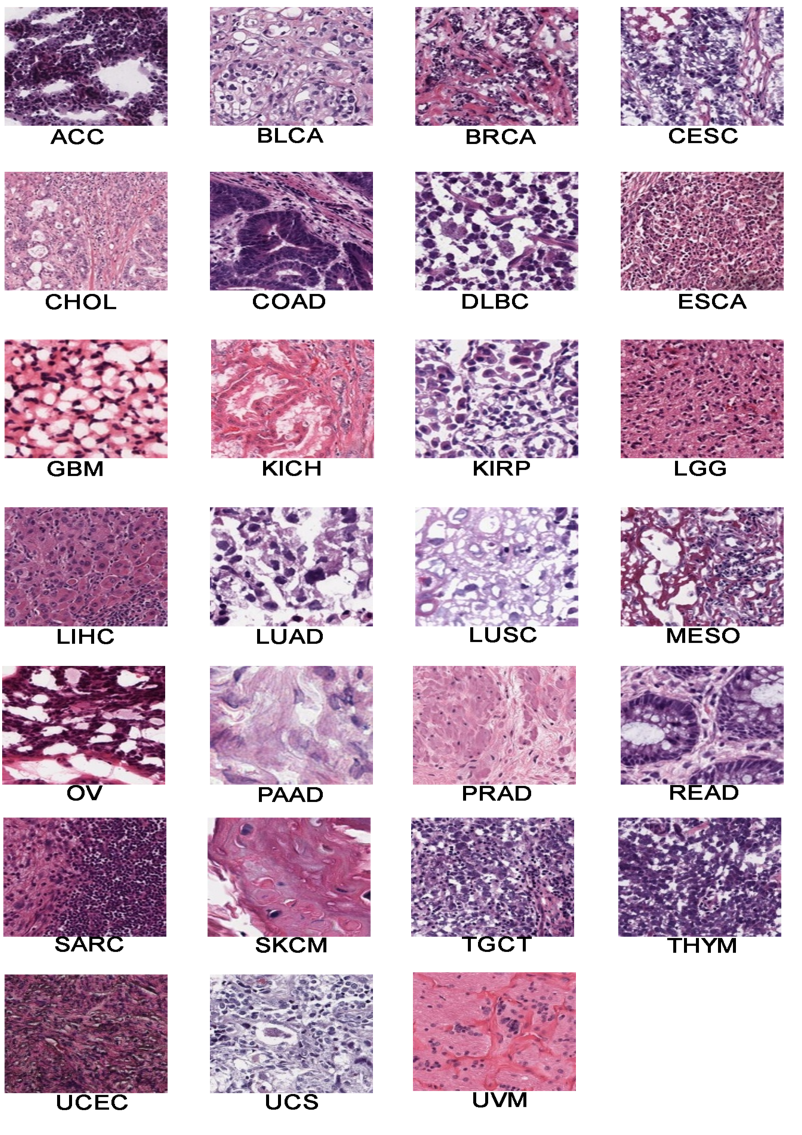
\includegraphics{figure/graphics-unnamed-chunk-19-1} 

}

\caption{A visual illustration of each disease state, based on sampled tile images.}\label{fig:unnamed-chunk-19}
\end{figure}

\end{document}
